\documentclass[12pt]{article}

\usepackage{pablo-devoir}
\usepackage[a5paper,margin=1cm]{geometry}

\pagestyle{empty}

\title{Fonctions Histogramme}
\date{07/01/15}
\classe{2\up{des}14}
\dsnum{DM 3}

\begin{document}

\maketitle

\begin{itemize}
  \item Faire un des deux exercices 1 et 2 au choix (l'exercice 1 est plus difficile).
  \item Les exercices 3 et 4 sont obligatoires.
\end{itemize}

\begin{exercice}[Variation de la fonction carrée]
  Le but de l'exercice est d'étudier les variations de la fonction $f:x\mapsto x^2$, définie sur $\mathbb{R}$ (appellée \emph{fonction carrée}).

  \begin{enumerate}
    \item Rappeler la définition de \emph{fonction croissante} et \emph{fonction décroissante}.
    \item 
      \begin{enumerate}
        \item Dans un repère orthonormé, tracer la courbe représentative de $f$, pour des abscisses allant de $-2$ à 2, et des ordonnées de $-4$ à 4.
        \item Par lecture graphique, conjecturer les variations de $f$.
      \end{enumerate}
    \item Soient $a$ et $b$ deux nombres positifs, tels que $a<b$.
      \begin{enumerate}
        \item Quel est le signe de $a+b$ ? Quel est le signe de $a-b$ ?
        \item En déduire le signe de $\left( a+b \right)\left( a-b \right)$.
        \item En déduire que $a^2<b^2$.
        \item En déduire le sens de variations de $f$ sur $\left[ 0; +\infty \right[$.
        \end{enumerate}
    \item Refaire le même raisonnement avec $a$ et $b$ deux nombres négatifs, et en déduire le sens de variations de $f$ sur $\left] -\infty;0 \right]$.
    \item Conclure en dressant le tableau de variations de $f$ sur $\mathbb{R}$.

  \end{enumerate}

\end{exercice}

\begin{exercice}[Variations d'une fonction affine]
  Le but de l'exercice est d'étudier les variations des fonctions $f:x\mapsto 3x-2$ et $g:x\mapsto -x+1$.
  \begin{enumerate}
    \item Rappeler la définition de \emph{fonction croissante} et \emph{fonction décroissante}.
    \item Tracer dans un repère orthonormé les courbes de $f$ et $g$, et donner leurs variations par lecture graphique.
    \item \emph{Étude de $f$.} Soient $a$ et $b$ deux nombres tels que $a<b$.
      \begin{enumerate}
        \item Compléter le raisonnement suivant avec les signes $<$ et $>$.
          \begin{align*}
            a &\ldots b\\
            3a & \ldots 3b\\
            3a-2 &\ldots 3b-2\\
            f(a) &\ldots f(b)
          \end{align*}
        \item En déduire le sens de variations de $f$.
      \end{enumerate}
    \item \emph{Étude de $g$.} Soient $a$ et $b$ deux nombres tels que $a<b$.
      \begin{enumerate}
        \item Compléter le raisonnement suivant avec les signes $<$ et $>$, et en justifiant le passage à la deuxième ligne.
          \begin{align*}
            a &\ldots b\\
            -a & \ldots -b \text{\hspace{1cm}car \ldots}\\
            -a+1 &\ldots -b+1\\
            g(a) &\ldots g(b)
          \end{align*}
        \item En déduire le sens de variations de $g$.
      \end{enumerate}
  \end{enumerate}
\end{exercice}

\begin{exercice}[Histogramme à classes irrégulières]
  Alain, intéressé par la météorologie, mesure les précipitations chez lui
  toutes les semaines. Il part quinze jours en vacances entre les 36\up{e} et 50\up{e} jour, et n'a donc pu faire qu'un seul relevé pour l'ensemble de ces deux semaines.
  
  ~

  \hspace{-2.5em}\begin{tabular}{p{2cm}||c|c|c|c|c|c|c}
    Jours &
    $\left[ 1; 8 \right[$ &
    $\left[ 8; 15 \right[$ &
    $\left[ 15; 22 \right[$ &
    $\left[ 22; 29 \right[$ &
    $\left[ 29; 36 \right[$ &
    $\left[ 36; 50 \right[$ &
    $\left[ 50; 57 \right[$ \\
    \hline
    Précipita\-tions (mm) & 15 & 14 & 14 & 16 & 17 & 31 & 16 \\
  \end{tabular}

  Le tableau se lit de la manière suivante : \emph{Sur l'ensemble des sept premiers jours, il est tombé 15~mm d'eau.}

  \begin{enumerate}
    \item \emph{Étude des jours 36 à 50.}
      \begin{enumerate}
        \item Calculer la hauteur moyenne d'eau tombée par jour du 29\up{e} au 36\up{e} jour, puis la hauteur moyenne d'eau tombée par jour du 36\up{e} au 50\up{e} jour.
        \item Est-il tombé beaucoup plus d'eau de 36\up{e} au 50\up{e} jour que pendant le reste de l'étude ?
      \end{enumerate}
  \end{enumerate}

  Afin de visualiser les précipitations, Alain trace l'histogramme suivant.

  \begin{center}
    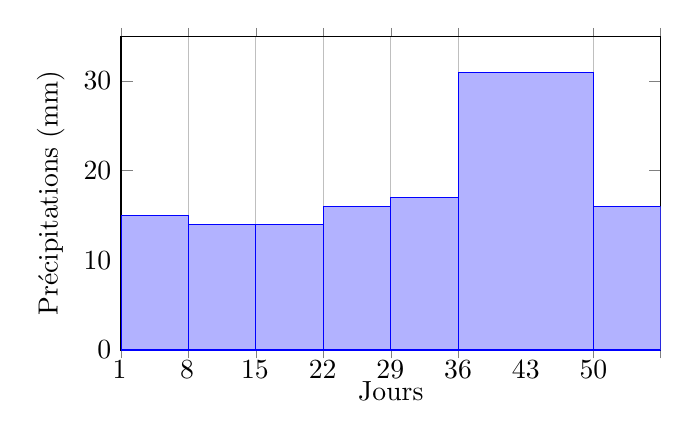
\begin{tikzpicture}
      \begin{axis}[
          yscale=0.7,
          ymin=0,
          ymax=35,
          xmin=1,
          xmax=57,
          xlabel={Jours},
          ylabel={Précipitations (mm)},
          ybar interval,
          xticklabel={~},
        ]
        \addplot coordinates {
          (1, 15)
          (8, 14)
          (15, 14)
          (22, 16)
          (29, 17)
          (36, 31)
          (50, 16)
          (57, 0)
        };
      \end{axis}
      \foreach \x in {1, 8, ..., 50} {
        \draw[thick] ({.12286*\x-0.1429}, 0) node[below]{\x};
    }
    \end{tikzpicture}
  \end{center}
  \begin{enumerate}
      \setcounter{enumi}{1}
    \item Selon son histogramme, pendant quels jours ont eu lieu les plus fortes précipitations ? Cela reflète-t-il la réalité (comparer cela avec le résultat de la question précédente) ?
  \end{enumerate}
  L'erreur d'Alain est qu'il a fait \emph{les hauteurs} des barres proportionnelles à
  la valeur des caractères, alors que \emph{les aires} des barres auraient dû être
  proportionnelles à la valeur des caractères.

  Le but de cet exercice est de tracer un histogramme correct.

  \begin{enumerate}
      \setcounter{enumi}{2}
    \item Dans cette question nous allons compléter le tableau de
      proportionnalité suivant, où les trois dernières lignes correspondent aux
      barres de l'histogramme que nous tracerons ensuite.

      \hspace{-3.5em}\begin{tabular}{p{2cm}||c|c|c|c|c|c|c}
    Jours &
    $\left[ 1; 8 \right[$ &
    $\left[ 8; 15 \right[$ &
    $\left[ 15; 22 \right[$ &
    $\left[ 22; 29 \right[$ &
    $\left[ 29; 36 \right[$ &
    $\left[ 36; 50 \right[$ &
    $\left[ 50; 57 \right[$ \\
          \hline
          \hline
          Précipita\-tions (mm) & 15 & 14 & 14 & 16 & 17 & 31 & 16 \\
          \hline
          \hline
          Aire &   & 28 & & & & \\
          \hline
          Largeur & 7 & 7& 7& 7& 7& 14& 7\\
          \hline
          Hauteur &&&&&&
        \end{tabular}

      \begin{enumerate}[(a)]
        \item Remplir la ligne « Aire », de sorte que l'aire soit
          proportionnelle aux précipitations.
        \item Remplir la ligne « Hauteur », de sorte que dans chaque colonne, le produit de la hauteur par la largeur soit égale à l'aire.
      \end{enumerate}
    \item Tracer l'histogramme en utilisant les largeurs et hauteurs des barres calculées dans le tableau.
    \item \emph{Application} Dans une étude de 2011 commandée par la \textsc{Hadopi} figurent les chiffres suivants, qui décrivent la somme moyenne dépensée chaque mois en produits et services culturels par les internautes ayant l'habitude de télécharger de manière illégale.

      \begin{center}
        \begin{tabular}{p{4cm}|c|c|c|c}
          Somme dépensée (\euro)
          & $\left] 0;20 \right[$
          & $\left[ 20;31 \right[$
          & $\left[ 31;100 \right[$
          & $\left[ 100;500 \right[$
          \\
          \hline
          Effectif
          & 342
          & 369
          & 250
          & 118
          \\
        \end{tabular}
      \end{center}
      Pour information (mais on ne représentera pas cette information sur le graphique), 237 personnes ont déclaré ne rien dépenser.

      Représenter ces données dans un histogramme.
  \end{enumerate}
\end{exercice}

\begin{exercice}[Histoire]
  Citer une mathématicienne, et dire pourquoi elle est connue.
\end{exercice}

\end{document}
